\documentclass[a4paper, 10pt]{article}
\usepackage[utf8x]{inputenc}
\usepackage[norsk]{babel}
\usepackage{natbib}
\usepackage{graphicx}
\usepackage[T1]{fontenc}
\usepackage{amsmath}
\usepackage{float}
\usepackage{mathtools}

\title{TDT4145 Øving 4}
\author{Kristoffer Dalby og Thor Martin Abrahamsen}
\date{}


\begin{document}

\maketitle

\thispagestyle{empty}
\newpage
\pagenumbering{arabic}
\setcounter{page}{1}

\section*{Oppgave 1}

\subsubsection*{a}
Supernøkkel er en samling av attributter hvor kombinasjonen av attributtene alltid vil være unik.\\
Nøkkel er en minimal supernøkkel, det vil si at du ikke kan fjerne en attributt og fortsatt ha en supernøkkel som er en unik kombinasjon.\\
Funksjonell avhengighet er en begrensning mellom to sett av attributter fra databasen. Det betyr at en attributt eller et sett med attributter bestemmer en annen attributt eller et annet sett med attributter\\

\subsubsection*{b}
Tillukningen av X er alle mulige funksjonelle avhengigheter som kan lages ut fra de funksjonelle avhengighetene som er gitt.\\

Algoritme:\\
Steg en, lag en liste med alle funksjonelle avhengigheter som er gitt.
Steg to, for alle avhengighetene gitt, hvis venstre side av avhengigheten er i listen og høyre siden ikke er, legg høyre side i listen.
Steg tre, Fortsett til listen ikke endress.

\subsubsection*{c}
$a+ = {a, e}$\\
$ab+ = {a, b, e, c, d}$\\
$e+ = {e}$

\subsubsection*{d}
Man finner en supernøkkel ved å analysere de funksjonelle avhengighetene. Dette er i allhovedsak beregning av tillukningene til kandidat settet for det vi lurer på om er en supernøkkel.
En supernøkkel er en nøkkel om den er minimal, det vil si at det ikke lenger kan fjernes attributter uten at den har supernøkkel status. Med andre ord, en nøkkel er en supernøkkel som er minimal.


\subsubsection*{e}
Hvis de like attributtene i begge de nye projeksjonene er supernøkkel utgjør en supernøkkel for begge projeksjonene vil har begge tabllene en tapsløs-join egenskap.

\subsubsection*{f}
$R1 \cap R2 = (bc) \neq R1 eller R2$ og er derfor ikke tapsløs.\\
$R1 \cap R2 = (bcd) = R2$ og er derfor tapsløs.\\
$R1 \cap R2 = (bc) = R2$ og er derfor tapsløs.\\


\subsubsection*{g}
Et relasjonskjema R er 3NF hvis alle ikke primærnøkkel attributter av R møter begge disse kravene:
\begin{itemize}
	\item Den er ikke en full funksjonell avhengighet av alle nøkler i R.
	\item Den er ikke transetiv for alle avhengigheter av alle nøkler i R.
\end{itemize}

\subsubsection*{h}
Dette er en god dekomponering, da den er tapsløs. Siden vi kan se at R3 er en relasjon mellom R1 og R2 og vi kan dermed finne alle attributtene.

\section*{Oppgave 2}

\subsubsection*{a}
Oppgaven oppgir at en student har en 4 byte nøkkel og en 4 byte blokkidentifikator som resulterer i 8 byte per student. En blokk har 4096 byte og vi bruker dette og den gjennomsnittlige fyllgraden av en blokk på 0.67 til å regne ut antall studenter per blokk.\\
$\frac{4096}{8} x 0.67 \approx 343$ som er antall studenter per blokk. Vi tar derretter å finner ut det totale antall blokker: \\
$\frac{200 000}{343} \approx 583$\\
Da blir det til slutt slik at det øverste nivået vil ha en blokk, som peker på to navigasjonsblokker under. Disse to blokkene vil peke på de resterende 583 blokkene. Dette fordi det kun er plass til 343 i en blokk.

\subsubsection*{b}
Det blir 6 diskaksesser, først vil vi lese rotnoden, etterfulgt av nivå en, søke gjennom blokkene, også skrive til løvnode og til slutt oppdatere nivå en noden og rotnoden. Blokkene vil ikke ligge bufferet i minne, men må leses fra disk.

\subsubsection*{c}
Ettersom vi kun skal oppdatere en node trenger vi ikke å oppdatere rotnoden og noden på nivå en. Dette gjør at vi totalt får fire diskaksesser. Vi antar også at systemet vår har harddisker med 4,5 ms søketid og solid state drives med 0,1 ms søketid.\\
Søketiden blir derfor $4.5 \times 4 \equiv 18 ms$ for harddisken og $0.1 \times 4 \equiv 0.4 ms$ for SSDen.

\subsubsection*{d}

\begin{figure}[H]
    \begin{center}
        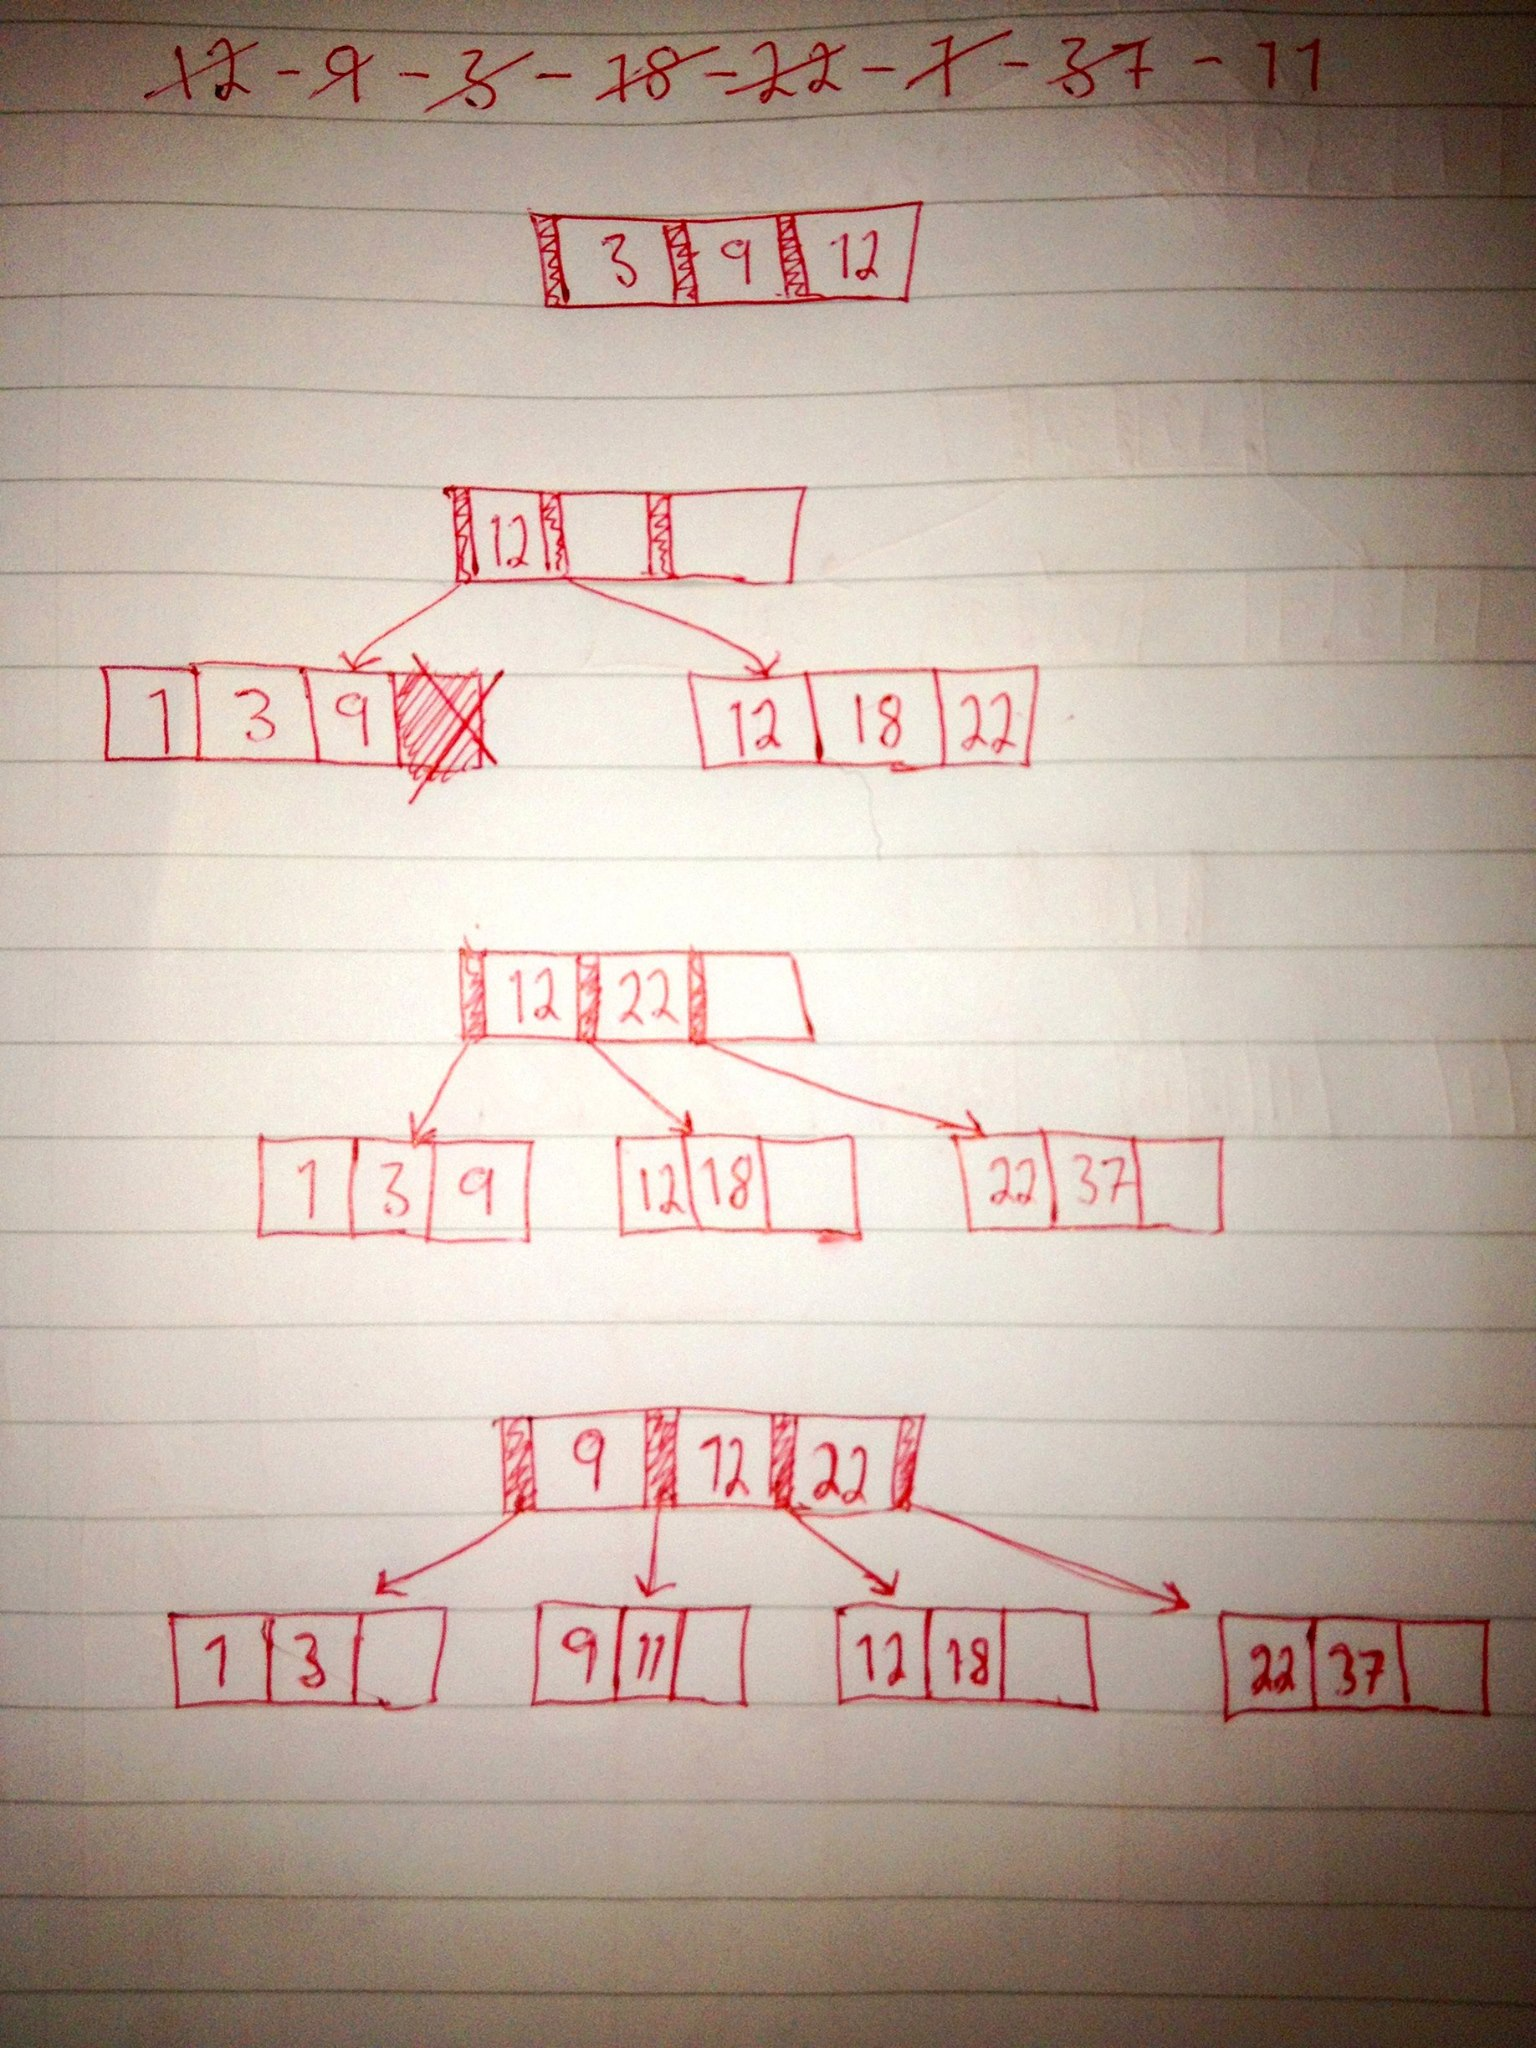
\includegraphics[width=7cm] {img/1891571_10153958793075161_6316017_o.jpg}
    \end{center}
\end{figure}

\section*{Oppgave 3}

\begin{figure}[H]
    \begin{center}
        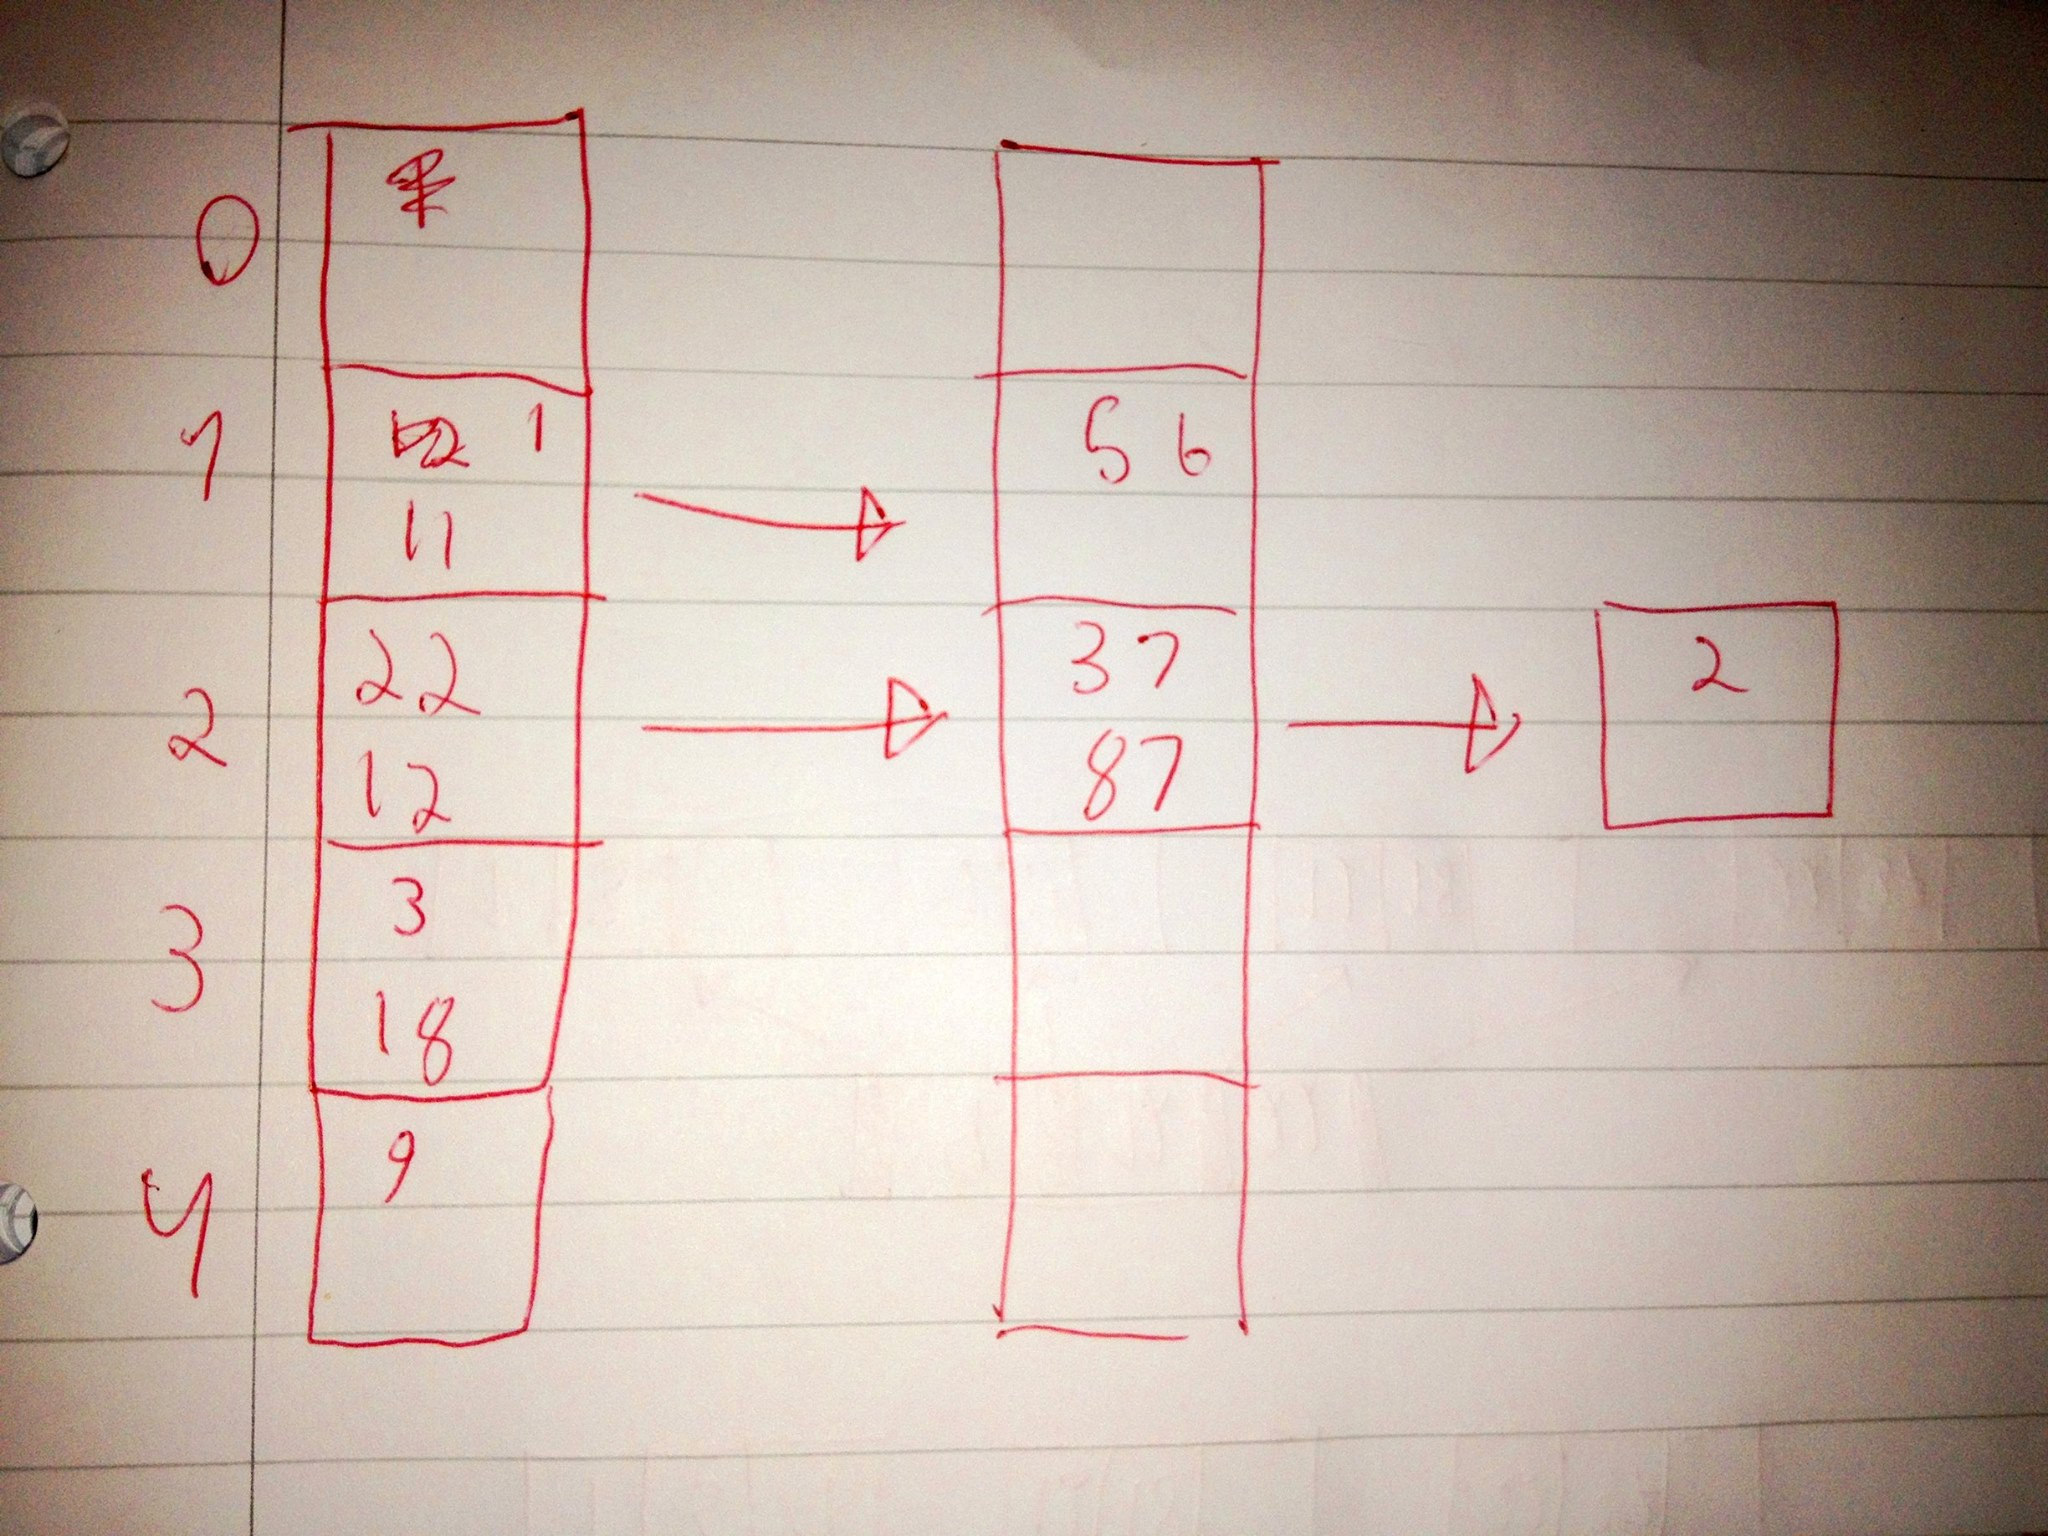
\includegraphics[width=7cm] {img/1493420_10153958793070161_995978780_o.jpg}
    \end{center}
\end{figure}

\newpage
\section*{Oppgave 4}
\subsubsection*{a}
Vi tolker utifra oppgaven at de spørringene i hovedsak vil vektlegge at vi kan bruke vinnavn som en nøkkel, vi ser derfor at hashing vil være å foretrekke ettersom oppslag i en hashtabell er svært raskt. Det vil i tilfelle også ikke være noe verre tilfelle en at man må søke sekvensielt hvis det er flere tabeller til nøkkelen.

\subsubsection*{b}
%Først finner vi ut det totale antall ansatte vi har plass til i hver blokk: \\
%$\frac{400 ansatte \times 100 bytes}{4096 bytes} \approx 10 $\\

%Deretter regner vi ut kostnadene vi får basert på antall operasjoner og antall blokker: \\
%Vi vet at p1 = 0.1, p2 = 0.5, p3 = 0.4 og at antall operasjoner er 2. Formelen er som følger:\\
%$(p1 + p2 + p3) \times ant ops \times ant blokk$\\
%$ (0.1 + 0.5 + 0.4) \times 2 \times 10 \equiv 20$\\

I oppgaven er det ikke oppgitt noen operasjoner på avdelingsrelasjonen. Vi antar også at det ikke derfor ikke gjøres noen store operasjoner på avdelinger, kanskje annet en en liten oppdatering i ny og ned og noen seleksjoner.\\

Vi ser at de mest vanlige spørringene er på ansatt-tabellen, med seleksjoner og innsettinger. Det gjøres sammenligninger på attributtene "personr", "navn" og "avdnavn" så det vil være hensiktsmessig å indeksere disse. ("navn" og "avdnavn" ettersom Q2 blir mest brukt). Vi ville benyttet en hash-indeks, optimalisert for direkteaksess og ekvivalensseleksjon.



\end{document}
